\documentclass[12pt]{article}
\usepackage[labelfont=bf,textfont=bf]{caption}
\usepackage{graphicx}
\usepackage{epstopdf}
\usepackage{microtype, color, amsmath, graphics, dcolumn, booktabs, multicol}
%\usepackage{natbib}
\usepackage[authoryear,square]{natbib}
\setcitestyle{citesep={,},aysep={}}
\usepackage{multirow}
\usepackage{enumitem}
\usepackage{bm}
\usepackage{MnSymbol}
\usepackage{amsfonts,dsfont}
\usepackage{setspace, lscape, longtable, rotating}
\usepackage{geometry}
\geometry{margin=1in}
\usepackage[normalem]{ulem}
\usepackage{appendix}
\usepackage{mathtools}
\usepackage{eurosym}
\usepackage{verbatim}
\DeclarePairedDelimiter{\ceil}{\lceil}{\rceil}
%\usepackage[nomarkers,nolists]{endfloat} %note, needs endfloat.cfg copied from efxmpl.cfg to work properly
%\renewcommand{\efloatseparator}{\mbox{}} %for endfloat
\newcommand{\putat}[3]{\begin{picture}(0,0)(0,0)\put(#1,#2){#3}\end{picture}}
\newcommand{\possessivecite}[1]{\citeauthor{#1}'s \citeyearpar{#1}}
%\usepackage{gaggl}
\widowpenalty=10000 \clubpenalty=10000 %keeps pdf open properties you like
\usepackage[bookmarks=false]{hyperref} 
\hypersetup{
	colorlinks=true,
	linkcolor=blue,
	filecolor=magenta,
	urlcolor=cyan,
	pdfauthor = {Nadav Tadelis}, 
 	pdftitle = {Reproducible Econometrics}, 
 	pdfsubject = {A reproducible approach to analyzing the effect of studying on grades},
	pdfborder =0 0 0, bookmarksopen=false, colorlinks=false,
%	pdfkeywords = {Keyword1, Keyword2, ...}, pdfcreator = {LaTeX with hyperref package}, pdfproducer = {dvips + ps2pdf}}
}
\usepackage{subcaption}
\newenvironment{changemargin}[2]{%
  \begin{list}{}{%
    \setlength{\topsep}{0pt}%
    \setlength{\leftmargin}{#1}%
    \setlength{\rightmargin}{#2}%
    \setlength{\listparindent}{\parindent}%
    \setlength{\itemindent}{\parindent}%
    \setlength{\parsep}{\parskip}%
  }%
  \item[]}{\end{list}} 
\linespread{1.3} 
%\doublespacing
\def\sym#1{\ifmmode^{#1}\else\(^{#1}\)\fi}

\newtheorem{claim}{Claim}
\newtheorem{definition}{Definition}

%Table Row Height
\usepackage{array}
\newcolumntype{M}[1]{>{\centering\arraybackslash}m{#1}}
\newcolumntype{N}{@{}m{0pt}@{}}

% Command for formatting inline code
\newcommand{\inlinecode}{\texttt}

% Changing the spacing above the footnote
\setlength{\skip\footins}{8mm}

% Changing spacing between multiple footnotes
\setlength{\footnotesep}{4mm}

% Graphics Path
%\usepackage{subfig}
\graphicspath{ {/Reproducible_Metrics/figures/} }

% ~~~~~ Temporary: Watermark ~~~~~~~
\usepackage{draftwatermark}
\SetWatermarkText{DRAFT}
\SetWatermarkScale{5}
\usepackage[dvipsnames]{xcolor}
% ~~~~~~~~~~~~~~~~~~~~~~~~~~~~~~

% For plotting functions
\usepackage{tikz}

% Custom functions for easy stats
\newcommand{\E}{\mathrm{E}}
\newcommand{\Cov}{\mathrm{Cov}}
\newcommand{\Var}{\mathrm{Var}}

\begin{document}

\title{Reproducibility and Applied Econometrics - The Effect of Studying on Grades\footnote{I would like to thank my thesis advisor, Professor Fernando P\'erez, for his support and insights, and Professor Maximilian Auffhammer for his generosity with his time.}}

\author{Nadav Tadelis}

\date{May 2018}


\pagenumbering{gobble} 

\maketitle

\hskip 80pt 


\begin{abstract}
In this paper we establish a framework for reproducible empirical research. We use a non-standard 2SLS model to estimate the marginal effects of studying on grades. The paper is split into two distinct sections. The first part is the econometric analysis on the causal impact of studying. The second part details the steps taken to ensure reproducibility and suggests how to easily integrate these methods into a researcher's future projects.

\vspace{3mm}
\noindent Git Repository: \url{https://github.com/nadavtadelis/Reproducible_Metrics}
\end{abstract}

\clearpage

\pagenumbering{arabic} 

%*******************************************************************************************************************
%*******************************************************************************************************************
\section{Introduction}
\label{sec_intro}
In recent years there has been a strong push to increase the reproducibility and replicability of scientific research. Unfortunately this movement seems to have been centered on the hard sciences and has not yet become standard practice in the social sciences. It is possible that this is partly due to a lack of reproducibly researched papers in these fields. This paper explores what responsible and reproducible research practices look like in applied econometrics. We present an instrumental variables approach to estimating the causal effect of studying on grades and develop custom python scripts to implement an unusual 2SLS set up that allows for nonlinearity in our endogenous predictor. The latter part of this work discusses the current state of reproducibility in econometric research, and explains in detail the techniques implemented in the analysis.

This paper was written as my honors thesis for undergraduate studies in statistics at UC Berkeley. \textcolor{BrickRed}{[Need to decide whether to keep this here or in the footnote] I would like to thank my thesis advisor, Professor Fernando P\'erez, for his support and insights, and Professor Maximilian Auffhammer for his generosity with his time}. Due to deadlines for submission I was unable to spend an appropriate amount of time on the econometric analysis, and will point out some of the weak points in my models (specifically the instruments). Any comments or suggestions would be greatly appreciated. 

The rough idea for the econometric analysis in the paper is adapted from an independent project I completed during my Junior year. In a subsequent class the project was modified and rebuilt in a reproducible fashion. Sarah Johnson created the original intermediate functions in \href{https://github.com/nadavtadelis/Reproducible_Metrics/blob/master/p3functions.py}{\textcolor{cyan}{\inlinecode{p3functions.py}}}, and the associated tests and Travis integration. Chitwan Kaudan created the original Makefile for running the individual Jupyter Notebooks. All aspects of those original analyses have been altered significantly, and the history of the alterations is fully documented in the commit history of the git repo.

\textcolor{BrickRed}{[Maybe more background here before we dive in?]}


%*******************************************************************************************************************
\newpage
\section{Data}
The \href{https://archive.ics.uci.edu/ml/datasets/Student+Performance#}{\textcolor{cyan}{data}} being used are from the public archive of UCI's machine learning repository and were collected by Paulo Cortez of the University of Minho, Portugal in the 2005 - 2006 academic year (\cite{data_paper}). The data were collected in two secondary schools in the Alentejo region of Portugal, using school reports and questionnaires. The data were cleaned to only include students for which all the variables are known - and a further 111 students were discarded because of mismatched information between the surveys and the school reports. The data come with a file containing attribute information which can be found \href{https://archive.ics.uci.edu/ml/datasets/Student+Performance#}{\textcolor{cyan}{here}}; these include school, course, and many individual level characteristics. The data include 649 students from a Portuguese Language course of study, and 395 students from a Mathematics course. 

\textcolor{BrickRed}{[Need more about data collection methods here? There isn't much description in the original paper, maybe this is enough?]}

%~~~~~~~~~~~~~~~~~~
\subsection{Data Exploration}
\textcolor{BrickRed}{[This section is very rough, needs work!]}

There is some pre-analysis data cleaning and exploration that we run, which can be found in the data exploration notebook - \href{https://nbviewer.jupyter.org/github/nadavtadelis/Reproducible_Metrics/blob/master/data_exploration.ipynb}{\textcolor{cyan}{nbviewer}}, \href{https://github.com/nadavtadelis/Reproducible_Metrics/blob/master/data_exploration.ipynb}{\textcolor{cyan}{git}}; some figures from this notebook are included in appendix \ref{appendix_figs} \textcolor{BrickRed}{[MAKE SURE TO INCLUDE THESE]}. The notebook contains the full data exploration process, as well as explanations and commentary detailing the figure generation process.

We draw attention to two attributes of special import: there are stark differences in the distributions of the data between the two schools, and across the two courses of study. The school level differences seem to be fairly consistent; perhaps the two schools have slightly different grading policies. However, the within school course level differences are highly variable; this is perhaps capturing the heterogeneity between students who choose Portuguese Language and Mathematics. This strongly suggests that even our simplest models should include controls for school to account for different policies, and should estimate the two courses as separate entities to account for different types of students.


%~~~~~~~~~~~~~~~~~~
\subsection{Data Issues} \label{data_issues}
\textcolor{BrickRed}{[Very Rough, needs a lot of work]}

As is often the case in the education space, the data have some large issues that must be considered. As any undergraduate taking their first econometrics course would point out, much of the data are stated preferences (as opposed to observed). Happily, the test scores and number of absences are provided by the schools, so we can be certain in their accuracy. The issue with self-reported data is the potential for inaccuracy. Even if a student is not maliciously providing misinformation, it is likely that personal biases are affecting the response. With variables like weekly hours of free time, this self reported data might actually be a benefit, as we are getting information about the student's perception of reality rather than the truth. If a student reports that they have very little free time then that tells us something about how they view their current time allocations. As such, these variables might be useful as controls for student level heterogeneity, but should be considered with a healthy dose of skepticism, and estimated coefficients should be interpreted with care. \textcolor{BrickRed}{[Think about this more.]} The issue of self reported data becomes more problematic when it comes to our variable of interest - hours of studying per week. While our central research goal is identifying a relationship between hours of studying and academic success, our data on hours of studying cannot be trusted as accurate \textcolor{BrickRed}{[expand more here]}.

In addition to the issue of self reporting, our data on studying time (and other variables) suffers from another issue; categorical mappings of quantitive measures. Many of the quantitive variables in the data are reported as categorical bins. For example, weekly studying time is coded as four distinct levels (0-2 hours, 2-5 hours, 5-10 hours, and 10+ hours). In the case of studying time, we explore two different re-mapping schemes\footnote{Mapping both as discrete and continuous, detailed in the data exploration notebook - \href{https://nbviewer.jupyter.org/github/nadavtadelis/Reproducible_Metrics/blob/master/data_exploration.ipynb}{\textcolor{cyan}{nbviewer}}, \href{https://github.com/nadavtadelis/Reproducible_Metrics/blob/master/data_exploration.ipynb}{\textcolor{cyan}{git}}}. But for the other variables with this format we treat them as categorical variables and include indicators for each level (thus allowing for some nonlinearity).
\textcolor{BrickRed}{[expand more here]}

Lastly, the data are cross-sectional rather than longitudinal, and the specific sampling time is unspecified. This is especially troubling in this setting because we are provided no information on when the student surveys were administered. Weekly studying time may change throughout the year, and may be partially determined by grades of previous examinations. If this is the case, and students update their studying allocation based on exam results, there is clear simultaneous causality between studying time and exam grades\footnote{A point explored more in section \ref{simul_caus}}. 
\textcolor{BrickRed}{[Do I need more here? Or is this enough of a brief intro to the later section?] - or should i just move the simultaneous causality section to here?}


%*******************************************************************************************************************
\newpage
\section{Models}
\textcolor{BrickRed}{[Do I need to focus more on the proxy model here?]}

We need to first set up our structural equation defining the relationship between grades and studying (\cite{CardKrueger}). Let an individual's grade be $g_i$ and weekly hours of studying be $s_i$ and their ``ability" be $a_i$. Then our model is:
$$
g_i = \beta_0 + \beta_1 s_i + \beta_2 s_i^2  + \beta_3 a_i + \bm{x}_{i,4:k}\bm{\beta}_{4:k} + \varepsilon_i
$$
Where $\bm{x}_{i,4:k}$ is a vector of school and course level characteristics and $\varepsilon_i$ captures some unobserved heterogeneity and disturbances. Note that grades are nonlinear in weekly study time. While this nonlinearity complicates our model, it seems necessary because assuming that marginal returns to studying must vary depending on the initial level of studying.

Clearly, there are issues with this model. How are we defining grades? The ideal set up would have a course specific set of simultaneous equations, where the number of equations is equal to the number of classes. The next best set up would involve estimating one equation for each type of class (quantitative, literary, historical, etc.) within each course. Another alternative would be to define grades as cumulative GPA. In this analysis, due to the limitations of the data, we define $g_i$ as the student's score on the final test for their course of study (G3 in the data).

Another issue with this model is: how are we defining ability? By its very nature, ability is unobserved. We can proxy for ability using other individual level characteristics (intelligence, age, parents' education, etc.) but we cannot fully capture ability because it does not have a clear measurable meaning. Hence, we must keep in mind that the model is never going to be fully specified.

We can think of a student's utility maximization problem as being some function of grades, free time (let's consider everything that is not studying, sleeping, or class as ``free time"), and studying time. We would expect that the coefficients on grades and free time would be positive, and the coefficient on study time would be negative, with magnitudes of these coefficients being determined by an individual's preferences. For example, a student who cares very little about grades, enjoys constantly partying, and hates studying, would have a small positive coefficient on grades, a large positive coefficient on free time, and a large negative coefficient on studying time\footnote{Of course, for some people and some subject matters of study, the coefficient on studying time may be positive with a decreasing marginal utility. We simplify the specification here dramatically.}. This student would maximize their utility and choose how to allocate their time, and would probably end up spending very little time studying. Notice that before maximizing their utility, an individual would replace grades with the previously defined model for grades (dependent on studying and ability); so someone who heavily values grades could end up having a positive coefficient on studying after including the model for grades into their utility function, even if they do not intrinsically value studying.

Establishing this utility function gives motivation for including variables that might introduce multicollinearity. For example, weekly amount of free time might not improve our estimate of the marginal effect of studying, and would be collinear with the amount of weekly studying. However, when we think of our observations as realizations of a decision making process that involves utility maximization over unobserved ability, there is an argument for including free time in the model estimation as a proxy for ability.

%~~~~~~~~~~~~~~~~~~
\subsection{Naive OLS}
\textcolor{BrickRed}{[Plots need finishing (better labels, axis names, titles for with/without controls, choose line type and color, etc.]} (maybe call them proxies here instead of controls because we call point out that they are proxies?) \textcolor{BrickRed}{[Maybe only include the first two plots in this section, and include the discontinuous mapping only in appendix?]}

In this section we discuss results from the naive model specifications we estimate in the model fitting 1 notebook -  \href{https://nbviewer.jupyter.org/github/nadavtadelis/Reproducible_Metrics/blob/master/model_fitting_1.ipynb}{\textcolor{cyan}{nbviewer}}, \href{https://github.com/nadavtadelis/Reproducible_Metrics/blob/master/model_fitting_1.ipynb}{\textcolor{cyan}{git}}. Below we plot studying time's estimated contribution to the final score (in percent).

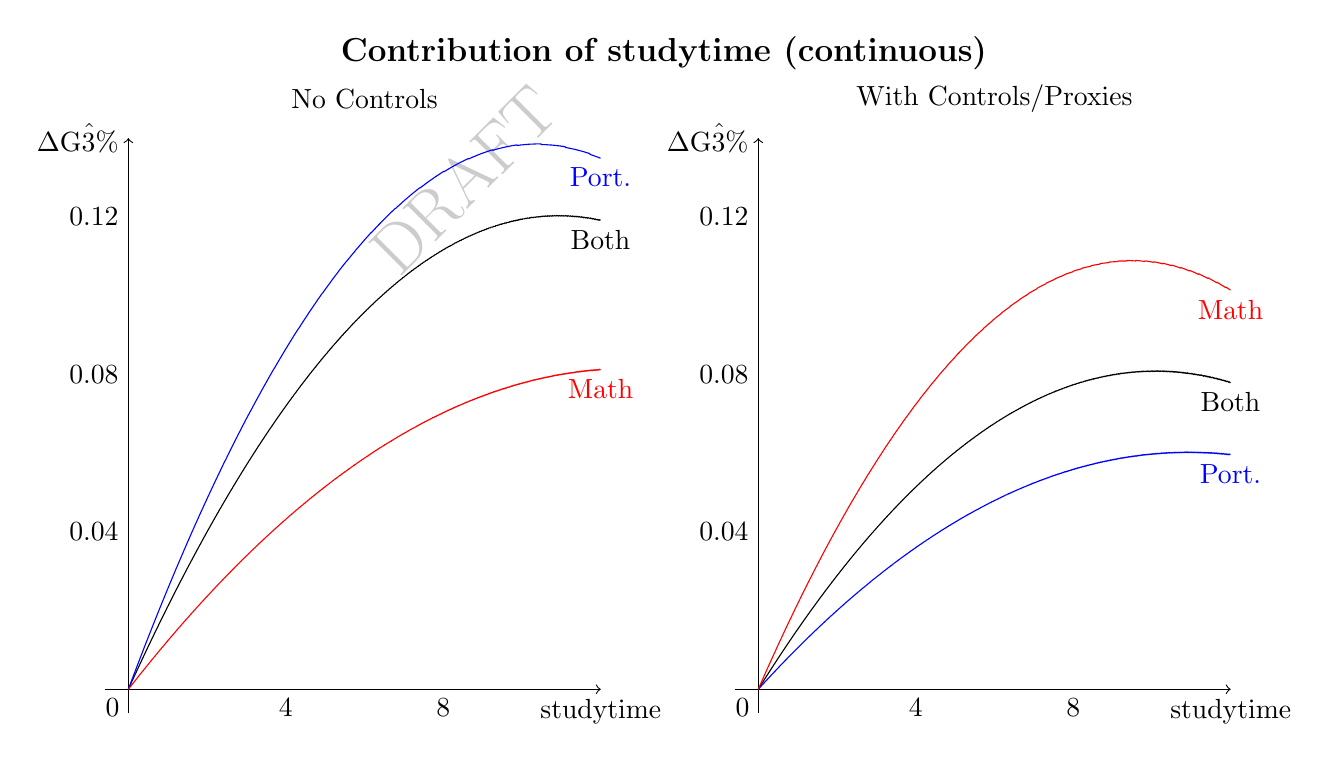
\begin{tikzpicture}
% Axis
\draw[->] (-0.3,0) -- (6,0) node[anchor=north] {studytime};
\draw[->] (0,-0.3) -- (0,7) node[anchor=east] {$\Delta\hat{\mathrm{G3}\%}$};

% labels
\draw	(-0.2,0) node[anchor=north] {0}
		(2,0) node[anchor=north] {4}
		(4,0) node[anchor=north] {8}
		(0,2) node[anchor=east] {0.04}
		(0,4) node[anchor=east] {0.08}
		(0,6) node[anchor=east] {0.12};

% Functions - WITHOUT CONTROLS
\draw[smooth, samples=1000, color=black, domain=0:6] plot ({\x},{50*(0.022*2*(\x) - 0.001*2*(\x)*2*(\x))}) 
        node[below] {Both}; %{$f(x) = t$};
\draw[smooth, solid, samples=1000, color=blue, domain=0:6] plot ({\x},{50*(0.0268*2*(\x) - 0.0013*2*(\x)*2*(\x))}) 
        node[below] {Port.};
\draw[smooth, solid, samples=1000, color=red, domain=0:6] plot ({\x},{50*(0.0128*2*(\x) - 0.0005*2*(\x)*2*(\x))}) 
        node[below] {Math};                  
% Title
\node[anchor=center] at (3, 7.5) {No Controls};
% Caption
%\node[anchor=center] at (3, -1) {Sub caption I};

\begin{scope}[xshift=8cm]
	% Axis
        \draw[->] (-0.3,0) -- (6,0) node[anchor=north] {studytime};
        \draw[->] (0,-0.3) -- (0,7) node[anchor=east] {$\Delta\hat{\mathrm{G3}\%}$};

	% labels
	\draw	(-0.2,0) node[anchor=north] {0}
			(2,0) node[anchor=north] {4}
			(4,0) node[anchor=north] {8}
			(0,2) node[anchor=east] {0.04}
			(0,4) node[anchor=east] {0.08}
			(0,6) node[anchor=east] {0.12};

	% Functions - WITH CONTROLS
\draw[smooth, samples=1000, color=black, domain=0:6] plot ({\x},{50*(0.016*2*(\x) - 0.0008*2*(\x)*2*(\x))}) 
        node[below] {Both};
\draw[smooth, solid, samples=1000, color=blue, domain=0:6] plot ({\x},{50*(0.0110*2*(\x) - 0.0005*2*(\x)*2*(\x))}) 
        node[below] {Port.};
\draw[smooth, solid, samples=1000, color=red, domain=0:6] plot ({\x},{50*(0.0229*2*(\x) - 0.0012*2*(\x)*2*(\x))}) 
        node[below] {Math};
% Titles
\node[above,font=\large\bfseries] at (current bounding box.north) {Contribution of studytime (continuous)};
\node[anchor=center] at (3, 7.5) {With Controls/Proxies};
% Caption
%\node[anchor=center] at (3, -1) {Sub caption II};        
\end{scope}
\end{tikzpicture}

\vspace{10pt} % REMOVE AFTER FORMATTING IS NICE AND FINALIZED

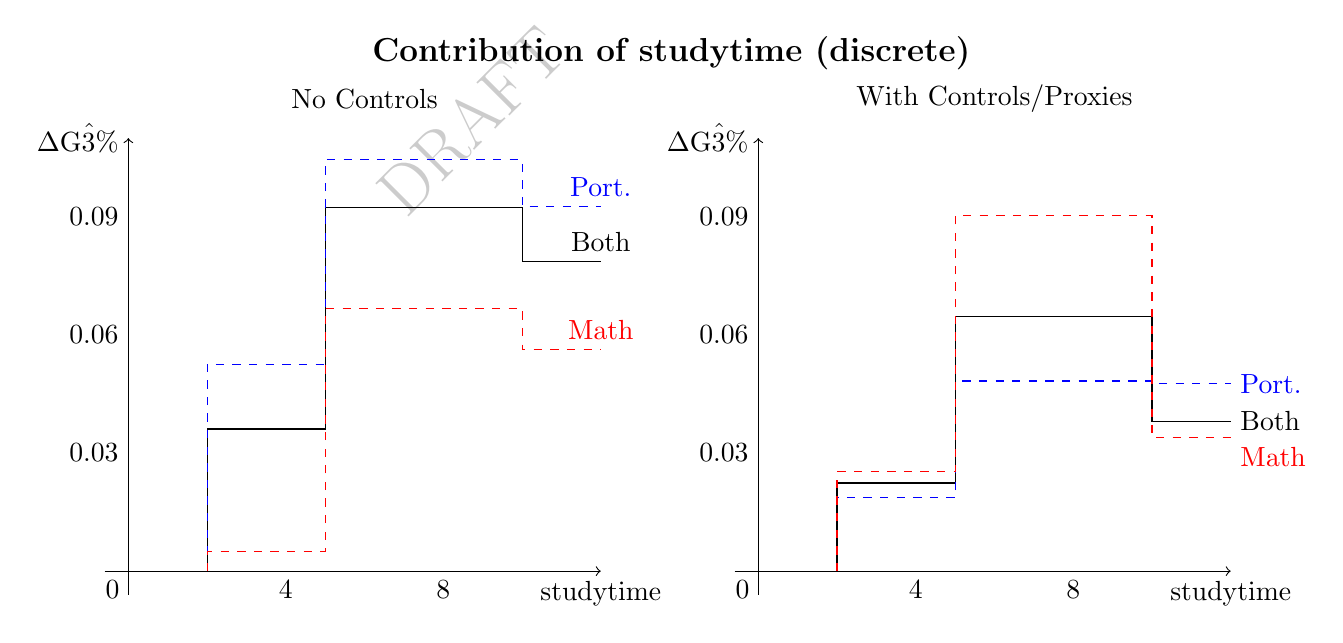
\begin{tikzpicture}
% Axis
\draw[->] (-0.3,0) -- (6,0) node[anchor=north] {studytime};
\draw[->] (0,-0.3) -- (0,5.5) node[anchor=east] {$\Delta\hat{\mathrm{G3}\%}$};

% labels
\draw	(-0.2,0) node[anchor=north] {0}
		(2,0) node[anchor=north] {4}
		(4,0) node[anchor=north] {8}
		(0,1.5) node[anchor=east] {0.03}
		(0,3) node[anchor=east] {0.06}
		(0,4.5) node[anchor=east] {0.09};

% Connected Segments - WITHOUT CONTROLS
\draw [color = black] (1,0) -- (1,50*0.0361) -- (2.5,50*0.0361) -- (2.5,50*0.0924) -- (5,50*0.0924) -- (5,50*0.0787) -- (6,50*0.0787)
	node[above] {Both}; 
\draw [color = blue, dashed] (1,0) -- (1,50*0.0526) -- (2.5,50*0.0526) -- (2.5,50*0.1045) -- (5,50*0.1045) -- (5,50*0.0927) -- (6,50*0.0927)
	node[above] {Port.}; 
\draw [color = red, dashed] (1,0) -- (1,50*0.005) -- (2.5,50*0.005) -- (2.5,50*0.0668) -- (5,50*0.0668) -- (5,50*0.0563) -- (6,50*0.0563)
	node[above] {Math};               
% Title
\node[anchor=center] at (3, 6) {No Controls};

\begin{scope}[xshift=8cm]
	% Axis
        \draw[->] (-0.3,0) -- (6,0) node[anchor=north] {studytime};
        \draw[->] (0,-0.3) -- (0,5.5) node[anchor=east] {$\Delta\hat{\mathrm{G3}\%}$};

	% labels
	\draw	(-0.2,0) node[anchor=north] {0}
			(2,0) node[anchor=north] {4}
			(4,0) node[anchor=north] {8}
			(0,1.5) node[anchor=east] {0.03}
			(0,3) node[anchor=east] {0.06}
			(0,4.5) node[anchor=east] {0.09};

	% Connected Segments - WITH CONTROLS
	\draw [color = black] (1,0) -- (1,50*0.0224) -- (2.5,50*0.0224) -- (2.5,50*0.0646) -- (5,50*0.0646) -- (5,50*0.0381) -- (6,50*0.0381)
		node[right] {Both};
	\draw [color = blue, dashed] (1,0) -- (1,50*0.0186) -- (2.5,50*0.0186) -- (2.5,50*0.0483) -- (5,50*0.0483) -- (5,50*0.0476) -- (6,50*0.0476)
		node[right] {Port.};
	\draw [color = red, dashed] (1,0) -- (1,50*0.0252) -- (2.5,50*0.0252) -- (2.5,50*0.0903) -- (5,50*0.0903) -- (5,50*0.0339) -- (6,50*0.0339)
		node[below right] {Math};        
% Titles
\node[above,font=\large\bfseries] at (current bounding box.north) {Contribution of studytime (discrete)};
\node[anchor=center] at (3, 6) {With Controls/Proxies};
\end{scope}
\end{tikzpicture}

%~~~~~~~~~~~~~~~~~~
\subsubsection{Additional Analysis}
In the model fitting 1 notebook we also include some additional explorations of the estimated models. We compute the variance inflation factor to check for multicollinearity (\cite{VIF, detecting}). We find slight collinearity between studying time and its square, but we are not worried about this collinearity because it is on our variable of interest, and the VIF is low enough to ignore. The rest of the collinearity that the VIF detects is so low that we don't need to consider it.

Additionally, we include a brief exploration of a LASSO-flavored penalization for variable selection (\cite{MLmetrics}) . We find that if we select a penalization parameter that shrinks all but seven of the coefficients to zero, the remaining coefficients are on studying time, school, course of study, number of failures, interest in higher education, mother's education, and whether the student is in the lowest bin of alcohol consumption. It is reassuring to see that the coefficient on studying time is not shrunk to zero. It is also nice to see that lasso shrinkage still retains mother's education, as this supports our previous discussion of including parental education despite some multicollinearity. We discuss the implications of the other non-zero coefficients in more detail in the model fitting 1 notebook -  \href{https://nbviewer.jupyter.org/github/nadavtadelis/Reproducible_Metrics/blob/master/model_fitting_1.ipynb}{\textcolor{cyan}{nbviewer}}, \href{https://github.com/nadavtadelis/Reproducible_Metrics/blob/master/model_fitting_1.ipynb}{\textcolor{cyan}{git}}.

%~~~~~~~~~~~~~~~~~~
\subsubsection{Simultaneous Causality} \label{simul_caus}
There is an additional issue with this model specification that was alluded to in section \ref{data_issues}. The data include three test scores: G1, G2, and G3. G1 and G2 are midterms, and G3 is the final. It is plausible that part of how students inform their study allocation decision comes from their results previous exams, and the how much time they studied for those exams\footnote{For example, if a student studied 5 hours a week leading up to the exam and received an 80\% she may choose to study for longer in the future in the hopes of increasing her grades.}. The data is taken at a single undefined point in time, so it is unclear when the students are reporting their weekly amount of studying. This complicates things; if the survey was administered after both midterms, then we may not expect their studying decision to change between the survey and the final, but if the survey was administered before either of the midterms then there is clear simultaneous causality between studying time, G1 and G2. Since we have only the single survey results with no time stamp, determining this relationship is intractable. With this limited information we must move forward either assuming that the reported studying times do not vary with mid term test results, or that the students were surveyed after both mid term results were released. These assumptions motivate the decision to exclude G1 and G2 from the model estimation.

%~~~~~~~~~~~~~~~~~~
\subsubsection{Endogeneity} \label{endogeneity}
In the second run of naive regressions we add many covariates as proxies representing unobserved ability (parental education, individual characteristics, and others detailed in the model fitting 1 notebook - \href{https://nbviewer.jupyter.org/github/nadavtadelis/Reproducible_Metrics/blob/master/model_fitting_1.ipynb}{\textcolor{cyan}{nbviewer}}, \href{https://github.com/nadavtadelis/Reproducible_Metrics/blob/master/model_fitting_1.ipynb}{\textcolor{cyan}{git}}). We pointed out that since ability is unobservable and undefinable we cannot expect to fully capture it through our proxies. Let $q_i$ be the unobserved portion of ability that we are not capturing through our imperfect proxies. Then we have:
$$
g_i = \beta_0 + \beta_1 s_i + \beta_2 s_i^2 + \beta_3 school_i + \beta_4 course_i + \beta_5 x_{i,5} + \cdots + \beta_k x_{i,k} + \gamma q_i + \nu_i
$$
Where $x_{i,5}, ..., x_{i,k}$ are proxies and $\nu_i$ is the structural error term. Let $x_{i,j}$ be the j'th covariate in the design matrix ($x_{i,1} = 1$, $x_{i,2} = s_i$, etc.) and let $\bm{x}_i$ be the vector of covariates for $i$. We are mainly interested in $\beta_1$ and $\beta_2$ the coefficients on studying. It is reasonable to assume that $\E[\nu_i | \bm{x}_i, q_i] = 0$ unfortunately we have no choice but to stick $q_i$ into the error term which gives us the new structural equation:
$$
g_i = \beta_0 + \beta_1 s_i + \beta_2 s_i^2 + \beta_3 school_i + \beta_4 course_i + \beta_5 x_{i,5} + \cdots + \beta_k x_{i,k} + \varepsilon_i
$$
Where $\varepsilon_i = \gamma q_i + \nu_i$. We know that $\nu_i$ is well behaved (uncorrelated with $x_{i,j} \forall j \in \{1,k\}$) but $\varepsilon_i$ is uncorrelated with the covariates iff $q_i$ is uncorrelated with the covariates. Lets look at the consistency of this set up (starting with the linear projection of $q_i$ onto $\bm{x}_i$):
\begin{align}
&g_i = \delta_0 + \delta_1 s_i + \delta_2 s_i^2 + \delta_3 school_i + \delta_4 course_i + \delta_5 x_{i,5} + \cdots + \delta_k x_{i,k} + \eta_i  \nonumber \\
&\E[\eta_i] = 0 \\
&\Cov[x_{i,j}, \eta_i] = 0
\end{align}
Where (1) and (2) follow from the definition of linear projections. Now we can represent our original model in terms of this linear projection:
\begin{alignat*}{2}
g_i &= {}&&\beta_0 + \beta_1 s_i + \beta_2 s_i^2 + \beta_3 school_i + \beta_4 course_i + \beta_5 x_{i,5} + \cdots + \beta_k x_{i,k} \\
      &     &&+ \gamma \delta_0 + \gamma \delta_1 s_i + \cdots + \gamma \delta_k x_{i,k} + \gamma \eta_i + \nu_i \\
g_i &=   &&(\beta_0 + \gamma\delta_0) + (\beta_1 + \gamma\delta_1)s_i + (\beta_2 + \gamma\delta_2)s_i^2 + \cdots + (\beta_k + \gamma\delta_k)x_{i,k} + \gamma \eta_i + \nu_i \\
      &\Rightarrow \ &&{} \E[\gamma\eta_i + \nu_i] = 0 \\
      &                    &&{} \Cov[x_{i,j}, \gamma\eta_i + \nu_i] = 0
\end{alignat*}
This shows that we can run OLS and get consistent estimates of $(\beta_j + \gamma\delta_j)$, but we are actually interested in $\bm{\beta}$. OLS does not allow us to recover $\bm{\beta}$ in this case because:
$$
\hat{\beta}_j \stackrel{p}{\longrightarrow} \beta_j + \underbrace{\gamma\delta_j}_{ \mathclap{\text{omitted variable bias}} }
$$
If $\gamma \ne 0$ and $\delta_j \ne 0$ then we cannot get a consistent estimate of $\beta_j$ using OLS. Rather, we get an endogenous estimator with a bias of $\gamma\delta_j$ (notice that the better our proxies identify ability, the smaller the bias term will be). Often times in practice researchers will assume that all $\delta_j$'s are zero except for the ones on the variables of interest. The implicit assumption behind setting $\delta_j = 0$ is that the unobserved $q_i$ and $x_{i,j}$ are independent (i.e. $\Cov[x_{i,j}, q_i] = 0$). In our setting this is actually a very reasonable assumption; we have already defined $x_{i,5}, ..., x_{i,k}$ as proxies for ability, meaning that the unobserved portion of ability should be orthogonal to each of these variables. It  is also reasonable to assume that there is independence between school and course level characteristics and the unobserved $q_i$. This simplifies\footnote{If we had only one endogenous variable we could simplify further because $\hat{\beta}_j \stackrel{p}{\longrightarrow} \beta_j + \gamma\frac{\Cov[x_j, q]}{\Var[x_j]}$. In this case we would be able to make some guesses about the direction of the bias.} our endogeneity problem so that the only endogenous variables are $s_i$ and $s_i^2$ ($\Cov[s_i, \varepsilon_i], \ \Cov[s_i^2, \varepsilon_i] \ne 0$). In the next sections we first give a brief overview of the instrumental variables approach to addressing endogeneity, and explain why standard two stage least squares is intractable in our setting. We then explore an instrumentation approach with nested generated regressors that may solve the problem.

%~~~~~~~~~~~~~~~~~~
\subsection{Q2SLS}
Lets first give a brief refresher of the instrumental variables approach to addressing endogeneity. In the last section we showed that for an endogenous variable $x_{i,j}$ OLS is no longer a consistent estimator for $\beta_j$. The instrumental variables approach allows us to solve the endogeneity problem. We require an instrumental variable $z_i$ which is observable and satisfies the following conditions:
\begin{spacing}{1}
\begin{enumerate}[label={(\arabic*)}]
	\item The instrument is uncorrelated with disturbances: $\Cov[z_i, \varepsilon_i] = 0$ \
	\item In the reduced form of $x_{i,j}$: $x_{i,j} = \phi_0 x_{i,1} + \phi_1 school_i + \cdots + \phi_{k-2}x_{i,k} + \theta_1 z_i + \vartheta_i$ the coefficient on our instrument is nonzero: $\theta_1 \ne 0$
	\item And $z_i$ is not one of our exogenous variables in the original estimation
\end{enumerate}
\end{spacing}
\noindent If $(1)-(3)$ hold, then we call $z_i$ a valid instrument for $x_{i,j}$. In settings with multiple valid instruments $\bm{z_1}, \bm{z}_2, ..., \bm{z}_M$ the standard procedure for identifying $\bm{\beta}$ is 2SLS. In the first stage of 2SLS we regress the endogenous variable $x_{i,j}$ on the exogenous variables and the instruments to get the fitted values $\hat{x}_{i,j} =  \sum_{k \ne j}\{\hat{\phi}_k x_{i,k}\} + \hat{\theta}_1 z_{i,1} + \cdots + \hat{\theta}_M z_{i,M}$. We use $\hat{x}_{i,j}$ as an estimate of the exogenous part of $x_{i,j}$ and in the second stage we regress our dependent variable on our exogenous variables and $\hat{x}_{i,j}$ to identify $\hat{\bm{\beta}}$. This approach can be easily extended to cases with multiple endogenous variables (where you would have as many first stage regressions as there are endogenous variables). However, with multiple endogenous variables, you must have at least as many instruments as endogenous variables, otherwise the fitted values would be collinear and the second stage estimators would lose consistency. In the next section we discuss issues with the 2SLS method in our setting.

%~~~~~~~~~~~~~~~~~~
\subsubsection{Motivation}
In section \ref{endogeneity} we established that the causal relationship between our grades and studying time is quadratic. This would usually not be a barrier to using 2SLS; the standard approach\footnote{Assuming only one instrument is available.} is to use the original instrument and its square as instruments in the two first stage equations (\cite{harmless}). However, this approach is unusable when the only instrument available is binary. In fact, even if we have multiple binary instruments it is not convincing to think that the exogenous portion of the squared endogenous variable will be correctly identified because interacting the binary instruments gives very little additional variation \textcolor{BrickRed}{[THINK ABOUT THIS MORE]}. Happily, Wooldridge suggests a variant of 2SLS that seems to address this issue of identifying a nonlinearly transformed variable with linear projection on binary variables.

%~~~~~~~~~~~~~~~~~~
\subsubsection{Estimation Procedure}
\textcolor{BrickRed}{[Or maybe this procedure section should be in merged into the above section? 'Motivation and Estimation']}

 The procedure that Wooldridge suggests is as follows (\cite{wooldridge}):
\begin{spacing}{1}
\begin{enumerate}[label={(\arabic*)}]
	\item \textit{First Stage:}
	\begin{enumerate}
		\item Regress the endogenous variable\footnote{In our model specification this is $s_i = x_{i,2}$} $x_{i,j}$ on the exogenous variables and the instruments to get fitted values $\hat{x}_{i,j}$
		\item Regress the endogenous variable squared\footnote{In our model specification this is $s_i^2 = x_{i,3}$} $x_{i,j}^2$ on the exogenous variables, the instruments, and the squared fitted values $(\hat{x}_{i,j})^2$. This gives fitted values for ${\wedge \atop x_{i,j}^2}$ 
	\end{enumerate} 
	\item \textit{Second Stage:} \\
	Regress the dependent variable on the exogenous variables and the two fitted values from the first stage ($\hat{x}_{i,j}$, ${\wedge \atop x_{i,j}^2}$)
\end{enumerate}
\end{spacing}
\noindent The intuition behind this model is that while using $(\hat{x}_{i,j})^2$ will not produce consistent coefficient estimates\footnote{Because the linear projection of the square is not the square of the linear projection, this mistake is known as the forbidden regression} for $\beta_j$; $(\hat{x}_{i,j})^2$ is still a square of the exogenous portion extracted from $x_{i,j}$ in part a of the first stage, and as such can be used as a valid instrument for $x_{i,j}^2$ \textcolor{BrickRed}{[NEED TO MAKE THIS MORE CLEAR]}. This should allow us to identify $\bm{\beta}$ even with the quadratic endogeneity and binary instrumentation.

%~~~~~~~~~~~~~~~~~~
\subsubsection{Properties of Q2SLS}
\textcolor{BrickRed}{[Explain the testing that I did for Q2SLS, mention that it looks like the coeff.s on endog\_sq\_hat and the exog vars are consistent and unbiased, but that the coeff on endog\_hat is consistent but biased. Point out the oddness of this behavior and note that I plan on researching this further.]} Note: pretty sure my instruments are weak (need to check), the simulation suggests that in the case of weak instruments the estimates are good but that the SE's are going to be large for the endogenous vars.

\textcolor{BrickRed}{[Discuss difficulty with finding the asymptotically consistent estimator for variance in Q2SLS because of the nested generated regressors]}

\textcolor{BrickRed}{[Give brief overview of bootstrapping and explain how its being used here to estimate variance of coeff. estimates in 2nd stage]} I think I'll need to explain that we report the coefficient estimates built on the full sample, rather than the average coefficients from the bootstrapping step - maybe link this back to the question of why the coefficient estimates are biased in the simulation, its not the same thing because here we are re-drawing and in simulation they are new draws, but it seems like there may be some connection here (maybe). Also add note about future integration of a wild bootstrap approach to variance estimation (stricter assumptions, but some really nice properties for endogenous models - see slide 15 from the link below)

\textcolor{BrickRed}{FOR BOOTSTRAPPING COV MATRIX:} See 8th slide of \href{https://www.math.kth.se/matstat/gru/sf2930/papers/wild.bootstrap.pdf}{\textcolor{cyan}{LINK}}. It also has notes on hypothesis testing and p values for bootstrapping with regression coefficients. SLIDE 14 HAS DISCUSSION OF BOOTSTRAPPING WITH ENDOGENOUS VARS!!

\textcolor{Red}{NOTE: this procedure only requires one instrument because the fitted vals from part a act as a second instrument so theres for sure no collinearity, this  means we could potentially only use one binary instrument!!! maybe this is the direction we should take rather than using a less than stellar second instrument. If this is the direction we go then I should repeat the function testing using binary instruments.}

%~~~~~~~~~~~~~~~~~~
\subsubsection{Application}
\textcolor{BrickRed}{[Discuss chosen instruments and give motivation for why they might be okay to use, give strong disclaimer that even if they are valid, they are probably weak instruments]} Justification for using 'going out' as instrument is stronger if we explain that we have controls for weekly and daily alcohol consumption (which is one thing that could affect grades through going out independently of studying time) so its a semi reasonable claim to say that going out is exogenous variation in available studying time once the detrimental effects of going out (namely drinking) are controlled for. not a super strong argument, but at least a little justification.

\textcolor{BrickRed}{[Report results]}

\textcolor{BrickRed}{[Discuss results]} Note: seems like we should expect that after identifying the causal effect we would see a decrease in the size of the coefficient on studying time because before that coefficient could have been positively biased because people who study more might also have a higher level of motivation of 'ability', so there might be a plausible intuitive argument that the size of the coeff should go down. need to think about this a bit more, but it might be worth mentioning.

Maybe: \textcolor{BrickRed}{[Reference appendix, and in the appendix include the results from Q2SLS with only 'essential' controls in the extra results subsection. Similar to the approach for the naive OLS at the beginning]}


%*******************************************************************************************************************
\newpage
\section{Reproducibility}
\textcolor{BrickRed}{[Need to clean up this section a lot]}

The importance of reproducible research has been understood for many years. In 1980 Thomas Mayer said ``Neither originality, logical rigor or any other criterion is ranked as `essential' by so many natural scientists as is replicability". Mayer was focusing on replicable research; unfortunately in the social science replicability is often far harder than reproducibility. When it takes five years and tens of thousands of dollars to collect the data for a single study, it is a difficult proposition to attempt to replicate the study from scratch. Additionally, it is unlikely that Mayer could have foreseen the degree to which data wrangling and programming would penetrate into academic research. This reliance on complex data pipelines and analysis with hundreds of dependencies makes replication a beast of a whole new nature. In the current state of empirical research, reproducing the results is half the battle. This opaqueness has led to many published papers that included results that were `p-hacked' or just included mistakes. Ensuring reproducibility would help alleviate many of these issues, and is a big step on the road to replicability.

Reproducibility has become especially important in the current political environment. The National Association for Scholars' recently published a report in which they advocate for use of the Secret Science Reformation Act (renamed the HONEST Act), which would forbid the Environmental Protection Agency from using any research that is not ``substantially reproducible" \cite{wired}. The NAS report goes even further and suggests that the bill should encompass all federal agencies and courts. Putting aside the various issues with the act\footnote{The act does not define ``substantially reproducible" with any rigor. It is possible that the flexibility of the act could lead to climate change deniers (and others) to call almost any study not substantially reproducible and bar federal agencies from acting on good research.}, if HONEST were to be expanded to other federal agencies, then policy-oriented research in the social sciences would be forced to adapt. Policy makers would need to see ``substantial reproducibility" before allowing a study to influence their policy decisions. Currently, very few empirical papers could be labeled as even somewhat reproducible, and part of the reason why might be that researchers believe implementing reproducible methods into their projects would be too costly in time and resources \cite{irreproducible}. Hopefully this paper provides a strong argument showing that conducting empirical research using reproducible methods is not only easy, but beneficial. And that were HONEST to be implemented to a wide degree, research need not be impeded\footnote{Ignoring the issue of data confidentiality.}.

%~~~~~~~~~~~~~~~~~~
\subsection{Current Resources}
\textcolor{BrickRed}{[Discuss current approaches to reproducibility in econometrics]}

\textcolor{BrickRed}{[Especially point out Gentzkow \& Shapiro's guide for research methods, and its helpfulness in ensuring that research workflow makes sense, but it's lack of open source reproducibility]}

%~~~~~~~~~~~~~~~~~~
\subsection{Basic Workflow}
\textcolor{BrickRed}{[Discuss git version control, environments, makefiles, using notebooks as a way to document any analysis that was not included in the final paper, but had an impact on the direction of the results (this increases confidence that there is not any unintentional p-hacking style things going on)]}
\textcolor{BrickRed}{[Definitely link to the stat 159 page because we don't want to go into the details of everything, just an overarching view of the tools and how they're used together. also summarize the benefits of some tools (ability to see edit history, ease of remote collaboration, ensuring compatibility on multiple machines, automatic function testing, etc.)]}

%~~~~~~~~~~~~~~~~~~
\subsection{Custom Functions}
\textcolor{BrickRed}{[Discuss the process of creating your own function in a way that other people can also use it without hassle: docstrings, comments, readability, etc.]}

\textcolor{BrickRed}{[Cover the process of testing a new function that isn't necessarily included in the final tests.py script (function\_testing.ipynb)]}

\textcolor{BrickRed}{[Explain Travis and CI]}

%~~~~~~~~~~~~~~~~~~
\subsection{Optional/Additional Elements}
\textcolor{BrickRed}{[Cover optional but useful things that the open source community has begun using: Binder, Sphinx, etc.] and discuss things I didn't have time to implement}

\textcolor{BrickRed}{[FOR SURE: mention that I did not have time to set up a way of porting the coeff.s and SE's directly from the notebooks to the tex file, and that ideally this would be fully automatic, so if the results changed in the jupyter notebook, then they would change in the tex file and the pdf (although since we are careful with the environments and version control, the coeffs should never change unless the model specifications change)]}


%*******************************************************************************************************************
\newpage
\section{Conclusion (? - maybe not needed)}
Maybe include a conclusion in the Q2SLS section, but not here.

%*******************************************************************************************************************
\newpage
\section{Appendix}

%~~~~~~~~~~~~~~~~~~
\subsection{Data Exploration Figures} \label{appendix_figs}
\textcolor{BrickRed}{[ONLY ONE FIGURE INCLUDED FOR NOW, NEED TO ADD OTHER FIGURES AND SCALE NICELY]}

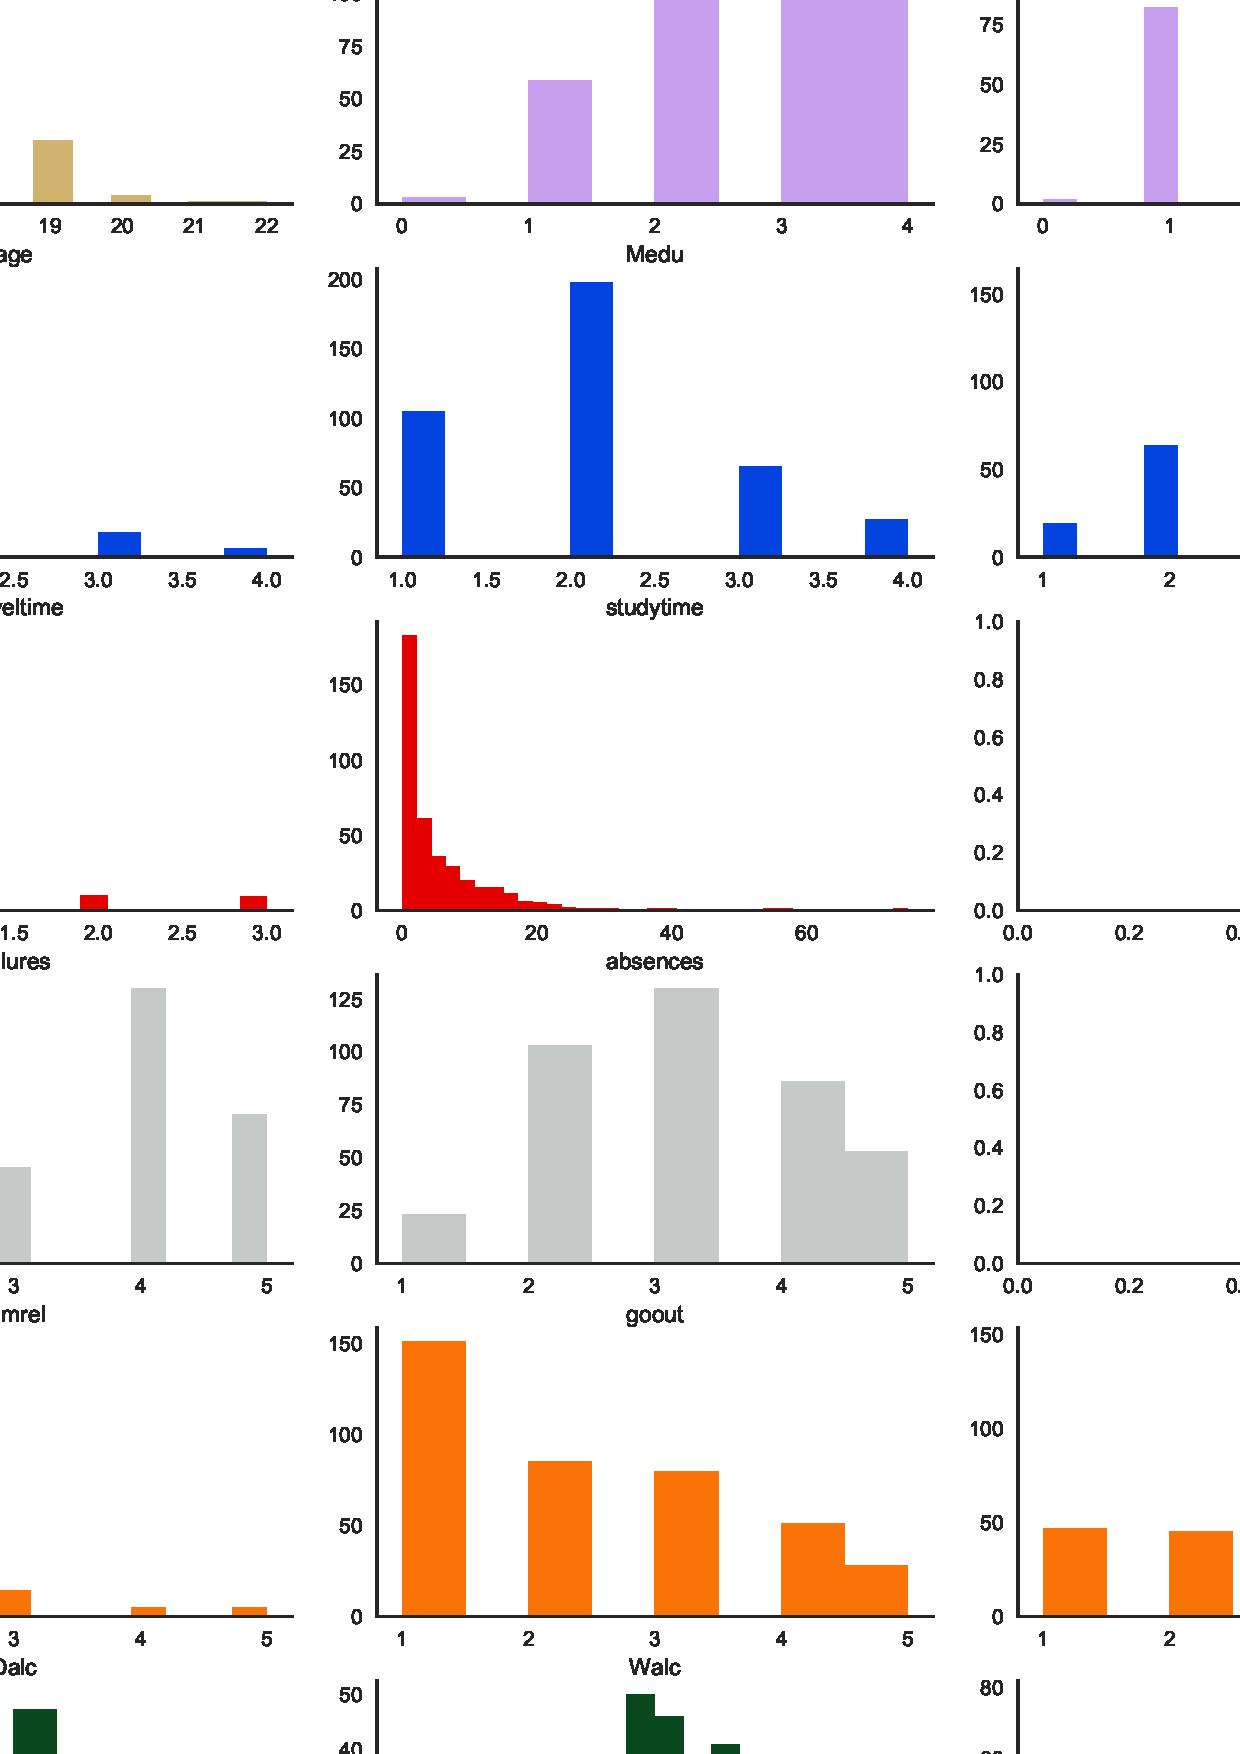
\includegraphics[scale=0.5]{figures/quantvar_hist_math.png}

%\begin{figure}[h]
%    \centering
%    {{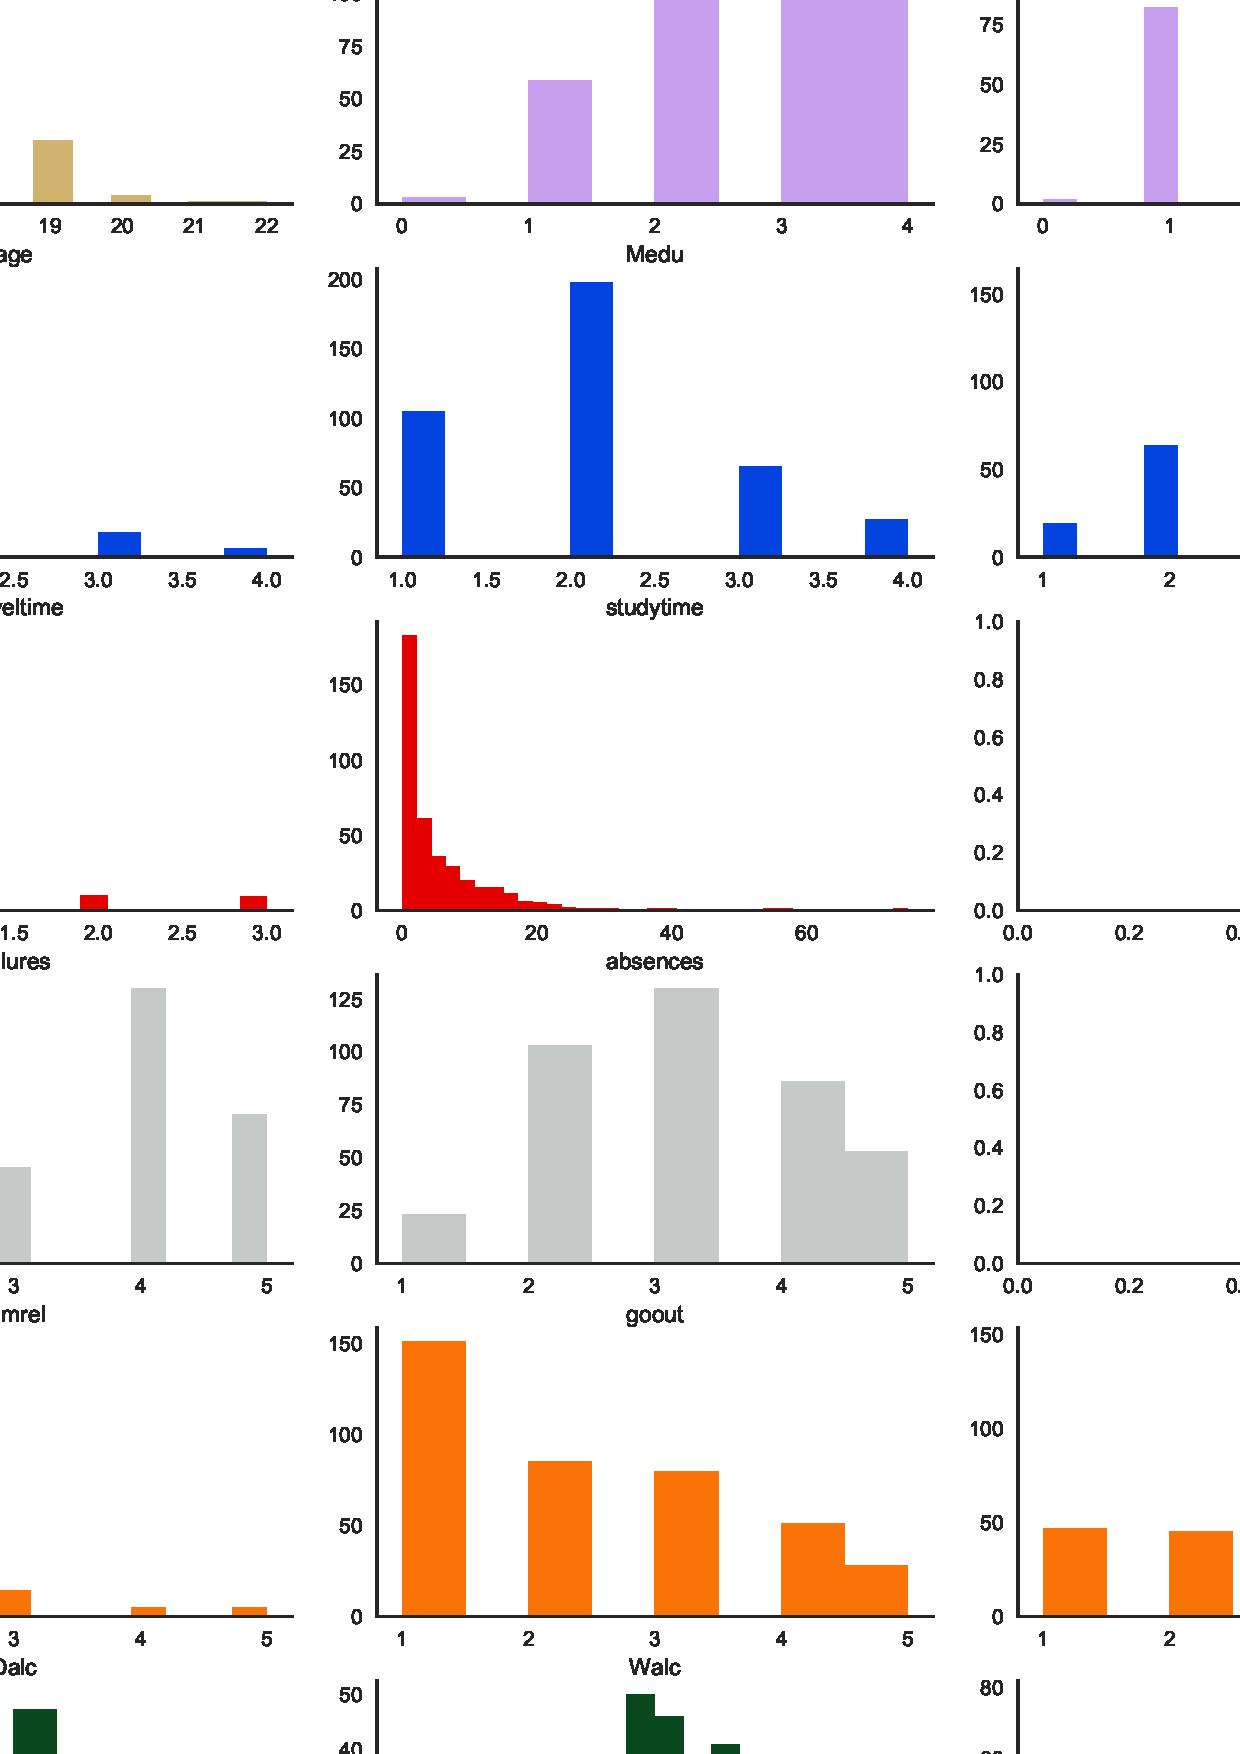
\includegraphics[width=10cm]{figures/quantvar_hist_math.png} }}
%    \\
%    {{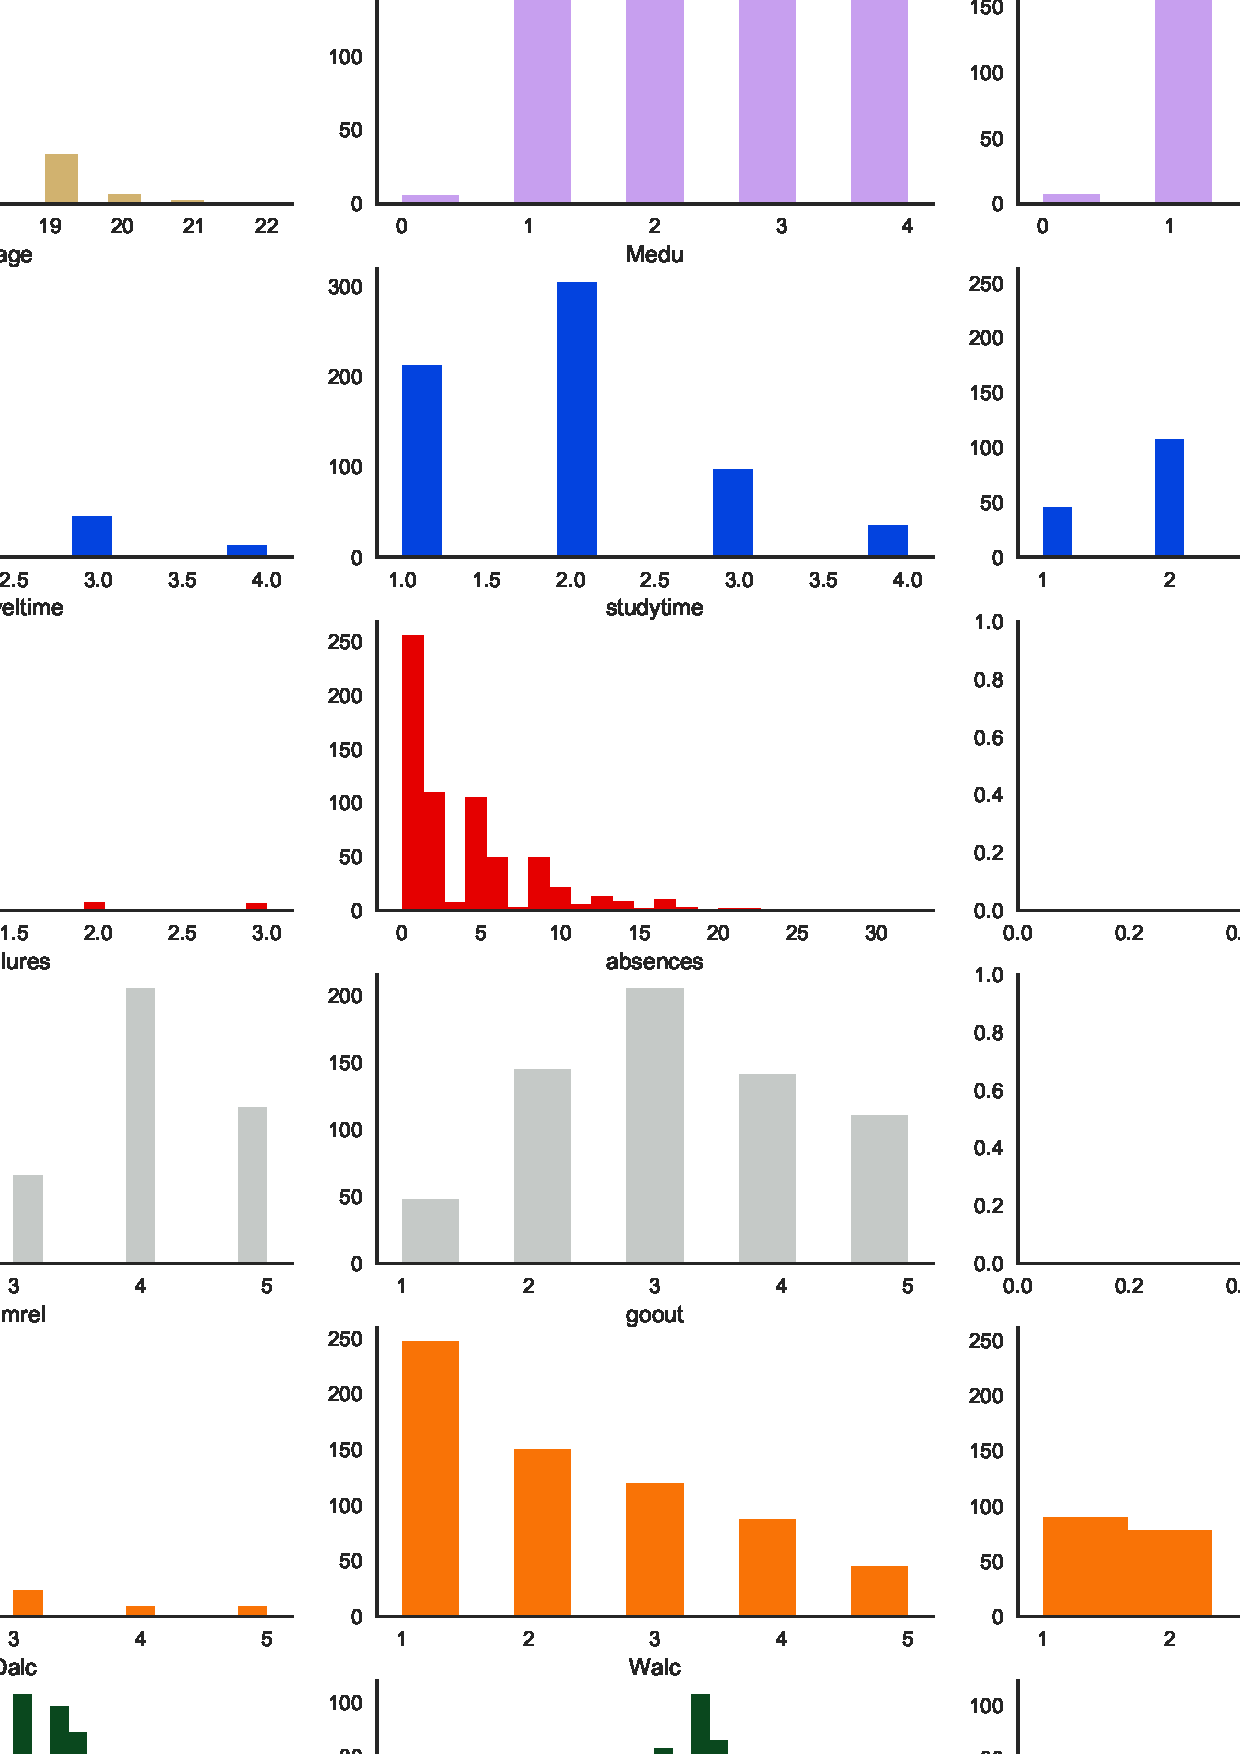
\includegraphics[width=7cm]{figures/quantvar_hist_por.png} }}
%    \caption{3 Figures arrayed}
%    \label{fig:example}
%\end{figure}

%~~~~~~~~~~~~~~~~~~
\subsection{Naive OLS Extra Models} \label{appendix_naive}

\textcolor{BrickRed}{[PUTTING ALL TABLES HERE FOR NOW BECAUSE HAVING TROUBLE PUTTING THEM IN SPECIFIC SECTION]}

QUESTION: \textcolor{BrickRed}{[Should we report these tables in the main paper and then report tables with all the covariates in the appendix? These would be extra long, and are viewable in the model fitting 1 notebook, so maybe it'd be better to just link to them?]}

\begin{table}[!h] \centering
  \caption{Naive OLS, Discrete Mapping}  
\resizebox{\columnwidth}{!}{%
\begin{tabular}{@{\extracolsep{0pt}}lD{.}{.}{-3} D{.}{.}{-3} D{.}{.}{-3}D{.}{.}{-3} D{.}{.}{-3} D{.}{.}{-3} } 
\\[-4ex]\hline 
\hline \\[-1.8ex] 
 & \multicolumn{6}{c}{\textit{Dependent variable:} G3 Grade (Percent)} \\%& \multicolumn{3}{c}{\textit{Dependent variable:} Screening2} \\ 
\cline{2-4} \cline{5-7}
\\[-1.8ex] & \multicolumn{1}{c}{\textit{Both}} & \multicolumn{1}{c}{\textit{Portuguese}} & \multicolumn{1}{c}{\textit{Mathematics}} & \multicolumn{1}{c}{\textit{Both}} & \multicolumn{1}{c}{\textit{Portuguese}} & \multicolumn{1}{c}{\textit{Mathematics}} \\ \ 
\\[-1.8ex] & \multicolumn{1}{c}{(1)} & \multicolumn{1}{c}{(2)} & \multicolumn{1}{c}{(3)} & \multicolumn{1}{c}{(4)} & \multicolumn{1}{c}{(5)} & \multicolumn{1}{c}{(6)} \\ 
\hline \\[-1.8ex] 
  Constant               & 0.5120^{***}  & 0.4942^{*** }  & 0.4784^{***}   & 0.4492^{***}     & 0.3136^{***}       & 0.8002^{***}         \\
                     	      & (0.0137)   & (0.0143)    & (0.0366)     & (0.1106)      & (0.1099)       & (0.2827)          \\ [1ex]  
  Studytime\_2     & 0.0361^{***}  & 0.0526^{***}   & 0.0050       & 0.0213        & 0.0181         & 0.0264           \\
                     & (0.0136)   & (0.0143)    & (0.0285)     & (0.0142)      & (0.0147)       & (0.0382)         \\[1ex]
 Studytime\_3     & 0.0924^{***}  & 0.1045^{***}   & 0.0668^{*}      & 0.0631^{***}     & 0.0474^{***}      & 0.0923^{**}         \\
                     & (0.0177)   & (0.0166)    & (0.0380)     & (0.0182)      & (0.0180)       & (0.0424)         \\[1ex]
 Studytime\_4     & 0.0787^{***}  & 0.0927^{***}   & 0.0563       & 0.0384        & 0.0481^{*}        & 0.0383           \\
                     & (0.0285)   & (0.0278)    & (0.0575)     & (0.0290)      & (0.0264)       & (0.0623)         \\[1ex]
 School\_GP           & 0.0742^{***}  & 0.0856^{***}   & 0.0283       & 0.0371^{**}      & 0.0602^{***}      & -0.0267          \\
                     & (0.0133)   & (0.0142)    & (0.0337)     & (0.0150)      & (0.0160)       & (0.0445)         \\[1ex]
 Course\_math         & -0.0954^{***} &             &              & -0.0958^{***}    &                &                  \\
                     		& (0.0128)   &             &              & (0.0150)      &                &                  \\[1ex] 
\hline \\[-1.8ex] 
 Proxies/Controls & \textit{no} & \textit{no} & \textit{no} & \textit{yes} & \textit{yes} & \textit{yes} \\[0.2ex]  
\hline \\[-1.8ex] 
Observations & \multicolumn{1}{c}{1,044} & \multicolumn{1}{c}{649} & \multicolumn{1}{c}{395} & \multicolumn{1}{c}{1,044} & \multicolumn{1}{c}{649} & \multicolumn{1}{c}{395} \\ 
Df & \multicolumn{1}{c}{5} & \multicolumn{1}{c}{4} & \multicolumn{1}{c}{4} & \multicolumn{1}{c}{68} & \multicolumn{1}{c}{67} & \multicolumn{1}{c}{67} \\
R$^{2}$ & \multicolumn{1}{c}{0.094} & \multicolumn{1}{c}{0.131} & \multicolumn{1}{c}{0.015} & \multicolumn{1}{c}{0.328} & \multicolumn{1}{c}{0.410} & \multicolumn{1}{c}{0.352} \\ 
Adjusted R$^{2}$ & \multicolumn{1}{c}{0.090} & \multicolumn{1}{c}{0.126} & \multicolumn{1}{c}{0.005} & \multicolumn{1}{c}{0.282} & \multicolumn{1}{c}{0.342} & \multicolumn{1}{c}{0.219} \\  
F Statistic & \multicolumn{1}{c}{24.62$^{***}$} & \multicolumn{1}{c}{22.95$^{***}$} & \multicolumn{1}{c}{1.469} & \multicolumn{1}{c}{7.23$^{***}$} & \multicolumn{1}{c}{5.91$^{***}$} & \multicolumn{1}{c}{2.74$^{***}$} \\ 
\hline 
\hline \\[-1.8ex] 
\textit{Note:}  & & & & \multicolumn{3}{r}{$^{*}$p$<$0.1; $^{**}$p$<$0.05; $^{***}$p$<$0.01} \\ 
\end{tabular} 
}
\end{table}


\begin{table}[!h] \centering
  \caption{Naive OLS, Continuous Mapping}  
\resizebox{\columnwidth}{!}{%
\begin{tabular}{@{\extracolsep{0pt}}lD{.}{.}{-3} D{.}{.}{-3} D{.}{.}{-3}D{.}{.}{-3} D{.}{.}{-3} D{.}{.}{-3} } 
\\[-4ex]\hline 
\hline \\[-1.8ex] 
 & \multicolumn{6}{c}{\textit{Dependent variable:} G3 Grade (Percent)} \\%& \multicolumn{3}{c}{\textit{Dependent variable:} Screening2} \\ 
\cline{2-4} \cline{5-7}
\\[-1.8ex] & \multicolumn{1}{c}{\textit{Both}} & \multicolumn{1}{c}{\textit{Portuguese}} & \multicolumn{1}{c}{\textit{Mathematics}} & \multicolumn{1}{c}{\textit{Both}} & \multicolumn{1}{c}{\textit{Portuguese}} & \multicolumn{1}{c}{\textit{Mathematics}} \\ \ 
\\[-1.8ex] & \multicolumn{1}{c}{(1)} & \multicolumn{1}{c}{(2)} & \multicolumn{1}{c}{(3)} & \multicolumn{1}{c}{(4)} & \multicolumn{1}{c}{(5)} & \multicolumn{1}{c}{(6)} \\ 
\hline \\[-1.8ex] 
  Constant          & 0.4879^{***}  & 0.4686^{***}   & 0.4572^{***}    & 0.4378^{***}    & 0.3049^{***}       & 0.7802^{***}         \\
                          & (0.0161)   & (0.0165)    & (0.0402)     & (0.1103)      & (0.1091)       & (0.2819)         \\[1ex]
  Studytime\_continuous     & 0.0220^{***}  & 0.0268^{***}   & 0.0128       & 0.0155^{***}     & 0.0107^{*}       & 0.0232^{*}          \\
                          & (0.0053)   & (0.0052)    & (0.0113)     & (0.0055)      & (0.0055)       & (0.0126)         \\[1ex]
  Studytime\_continuous\_sq & -0.0010^{***} & -0.0013^{***}  & -0.0005      & -0.0008^{**}     & -0.0004        & -0.0012          \\
                          & (0.0004)   & (0.0004)    & (0.0007)     & (0.0004)      & (0.0003)       & (0.0008)         \\[1ex]
  School\_GP                & 0.0737^{***}  & 0.0856^{***}   & 0.0262       & 0.0371^{**}      & 0.0603^{***}      & -0.0270         \\
                          & (0.0133)   & (0.0142)    & (0.0335)     & (0.0150)      & (0.0160)       & (0.0445)         \\[1ex]
  Course\_math              & -0.0956^{***} &             &              & -0.0959^{***}    &                &                  \\
                          & (0.0128)   &             &              & (0.0150)      &                &                  \\[1ex]
\hline \\[-1.8ex] 
 Proxies/Controls & \textit{no} & \textit{no} & \textit{no} & \textit{yes} & \textit{yes} & \textit{yes} \\[0.2ex]  
\hline \\[-1.8ex] 
Observations & \multicolumn{1}{c}{1,044} & \multicolumn{1}{c}{649} & \multicolumn{1}{c}{395} & \multicolumn{1}{c}{1,044} & \multicolumn{1}{c}{649} & \multicolumn{1}{c}{395} \\
Df & \multicolumn{1}{c}{5} & \multicolumn{1}{c}{4} & \multicolumn{1}{c}{4} & \multicolumn{1}{c}{68} & \multicolumn{1}{c}{67} & \multicolumn{1}{c}{67} \\ 
R$^{2}$ & 0.09       & 0.13        & 0.01         & 0.33          & 0.41           & 0.34             \\ 
Adjusted R$^{2}$ & 0.09       & 0.13        & 0.00         & 0.28          & 0.34           & 0.22             \\ 
F Statistic & 30.11^{***}      & 30.61^{***}       & 1.41         & 7.29^{***}          & 6.03^{***}           & 2.97^{***} \\ 
\hline 
\hline \\[-1.8ex] 
\textit{Note:}  & & & & \multicolumn{3}{r}{$^{*}$p$<$0.1; $^{**}$p$<$0.05; $^{***}$p$<$0.01} \\ 
\end{tabular} 
}
\end{table}

\newpage %%%% REMOVE THIS NEWPAGE AFTER FIGURE OUT HOW TO PUT TABLES WHERE WANTED %%%%

%~~~~~~~~~~~~~~~~~~
\subsection{Q2SLS Function Testing Procedure} \label{appendix_function_testing}
\textcolor{BrickRed}{[Can use some of the markdown from the functions testing notebook here, and obv.s link to the notebook as well]}

%~~~~~~~~~~~~~~~~~~
\subsection{Q2SLS Extra Models} \label{appendix_q2sls}

%~~~~~~~~~~~~~~~~~~
\subsection{Miscellanea (?)}

%*******************************************************************************************************************
\newpage

\singlespacing
\bibliographystyle{agsm}
\nocite{*} % makes sure that all items in .bib are included in bibliography, even if they aren't cited
\bibliography{tex_stuff/RM_bibliography}

%*******************************************************************************************************************

\end{document}




















